% !TEX program = xelatex

\documentclass[hidelinks, 12pt, a4paper]{article}

\usepackage{fontspec}
\setmainfont[Ligatures=TeX]{Linux Libertine O}

\usepackage[hidelinks, colorlinks = true, urlcolor = blue]{hyperref}

\usepackage{indentfirst}
\usepackage{graphicx}
\usepackage[left=2cm,right=2cm,top=2cm,bottom=2cm]{geometry}
\usepackage{lipsum}

%\setlength{\parindent}{1em}
%\setlength{\parskip}{1em}\title{Εργασία Στατιστικής}

%\title{Java socket programming \\ 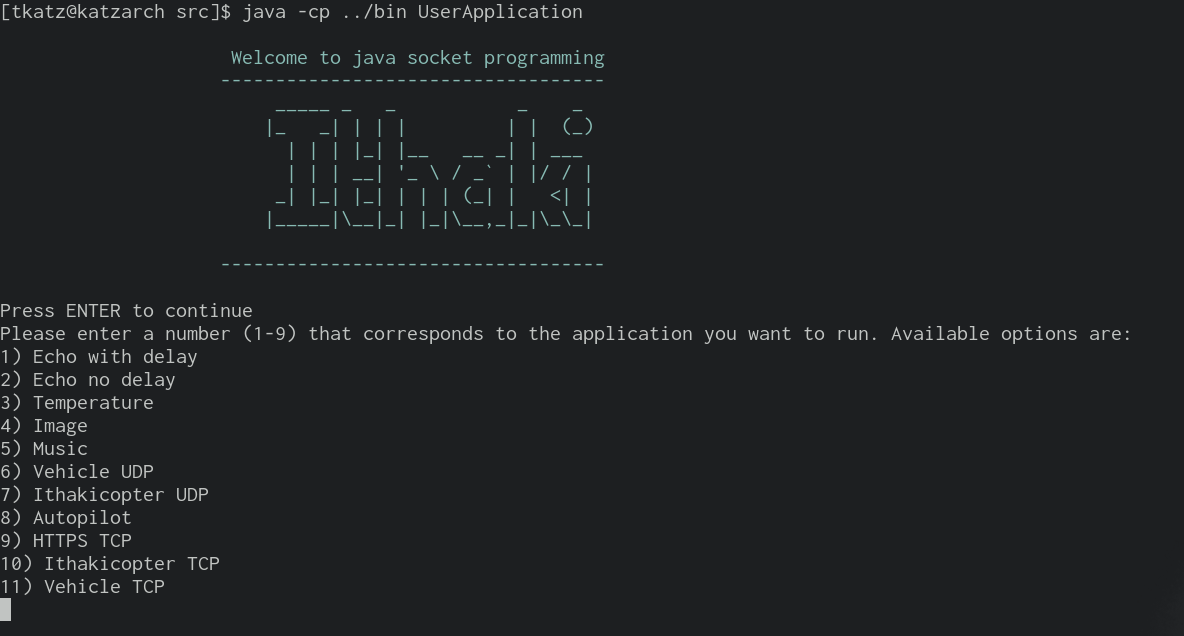
\includegraphics[width=\textwidth]{assets/login.png}}
% \author{Θεόδωρος Κατζάλης \\ ΑΕΜ:9282 \\ katzalis@auth.gr}
% \date{19/07/2020}

\begin{document}

\begin{titlepage}

\begin{figure}[h!]
  \begin{center}
    
\includegraphics[width=3cm]{assets/auth.pdf}
    \label{fig:cover_auth_logo}
  \end{center}
\end{figure}

\centering
\Large Αριστοτέλειο Πανεπιστήμιο Θεσσαλονίκης\\
\Large Πολυτεχνική Σχολή\\
%\large Τμήμα Ηλεκτρολόγων Μηχανικών και Μηχανικών Υπολογιστών\\
%\large Τομέας Τηλεπικοινωνιών

\vspace{\fill}

\LARGE \textbf{Java socket programming} \\
\LARGE \textbf{Δίκτυα 2}

\vspace{\fill}

\Large Θεόδωρος Κατζάλης \\
\Large ΑΕΜ:9282 \\ 
\Large katzalis@auth.gr

\vspace{\fill}
\raggedright

\centering
\vspace{\fill}
\today

\end{titlepage}

%\maketitle


\pagebreak
\tableofcontents
\pagebreak

% \section{Lorem}
% \lipsum


\section{G1}

\begin{figure}[h!]
\centering
	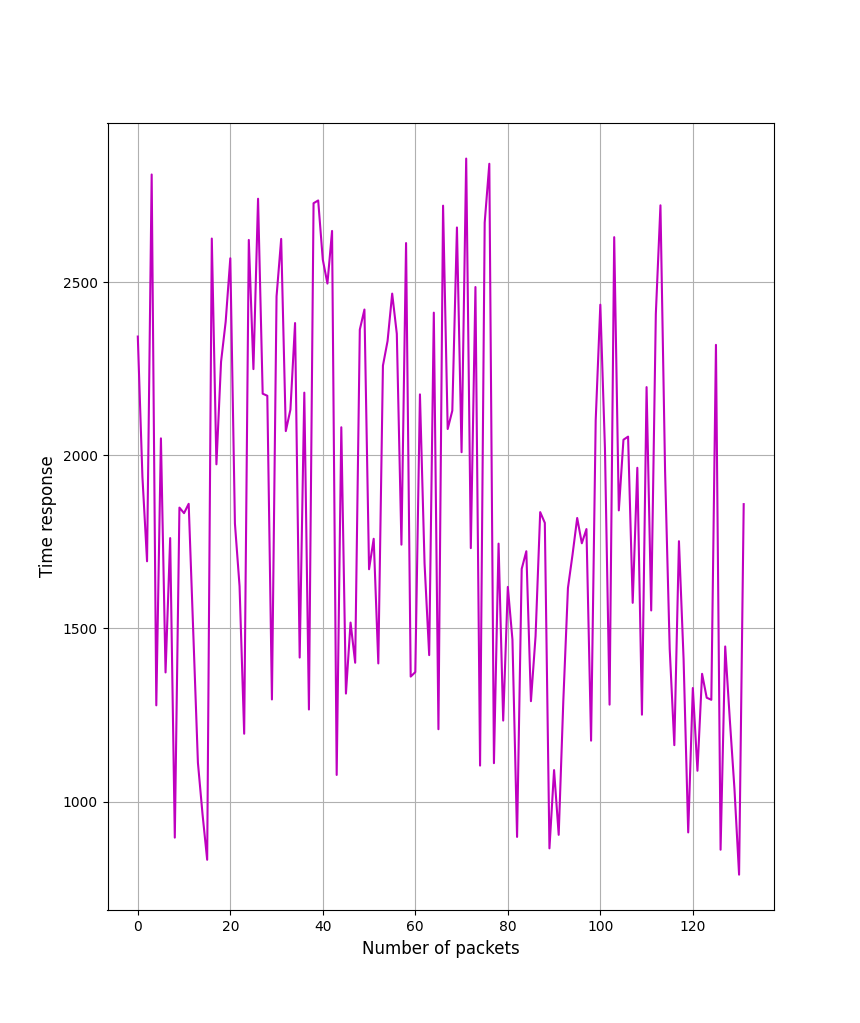
\includegraphics[height=.38\textheight, width=\textwidth]{assets/session1/g1.png}
	\caption{G1. 25/11/2020 22:32-22:36 Echo request code: E8142} 
\end{figure}

\section{G2}

\begin{figure}[h!]
\centering
	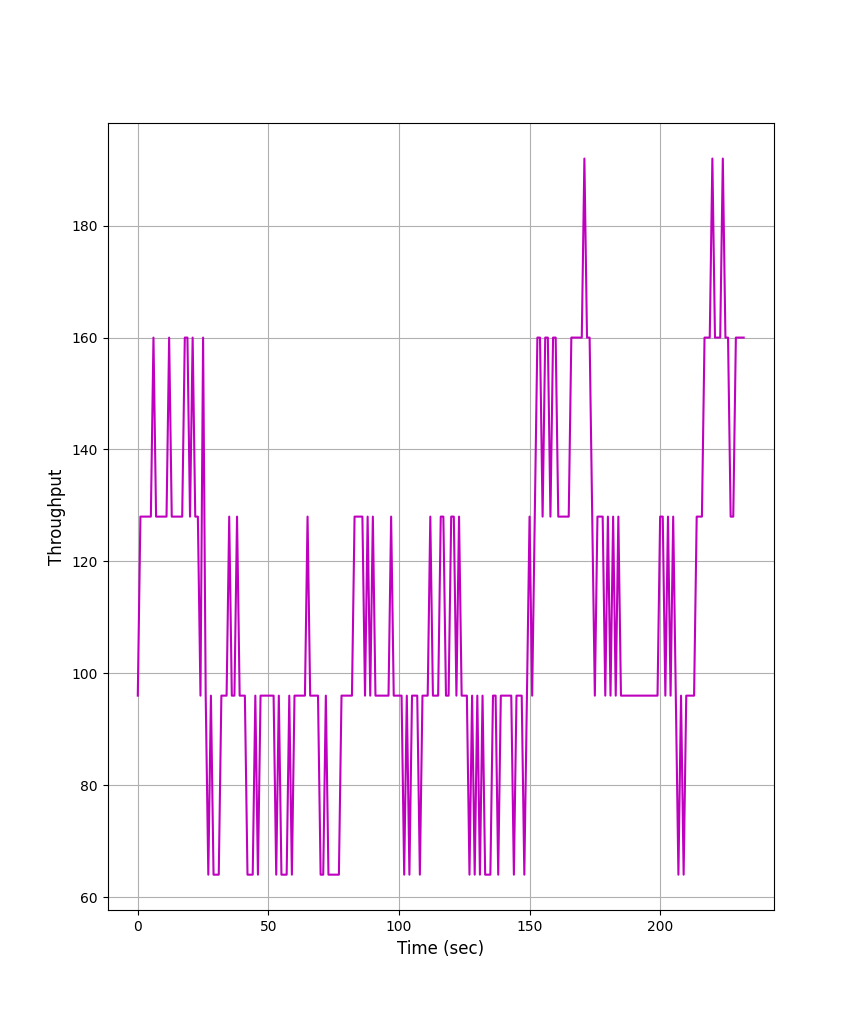
\includegraphics[height=.38\textheight, width=\textwidth]{assets/session1/g2.png}
	\caption{G2} 
\end{figure}

%\pagebreak

\section{G3}

\begin{figure}[h!]
\centering
	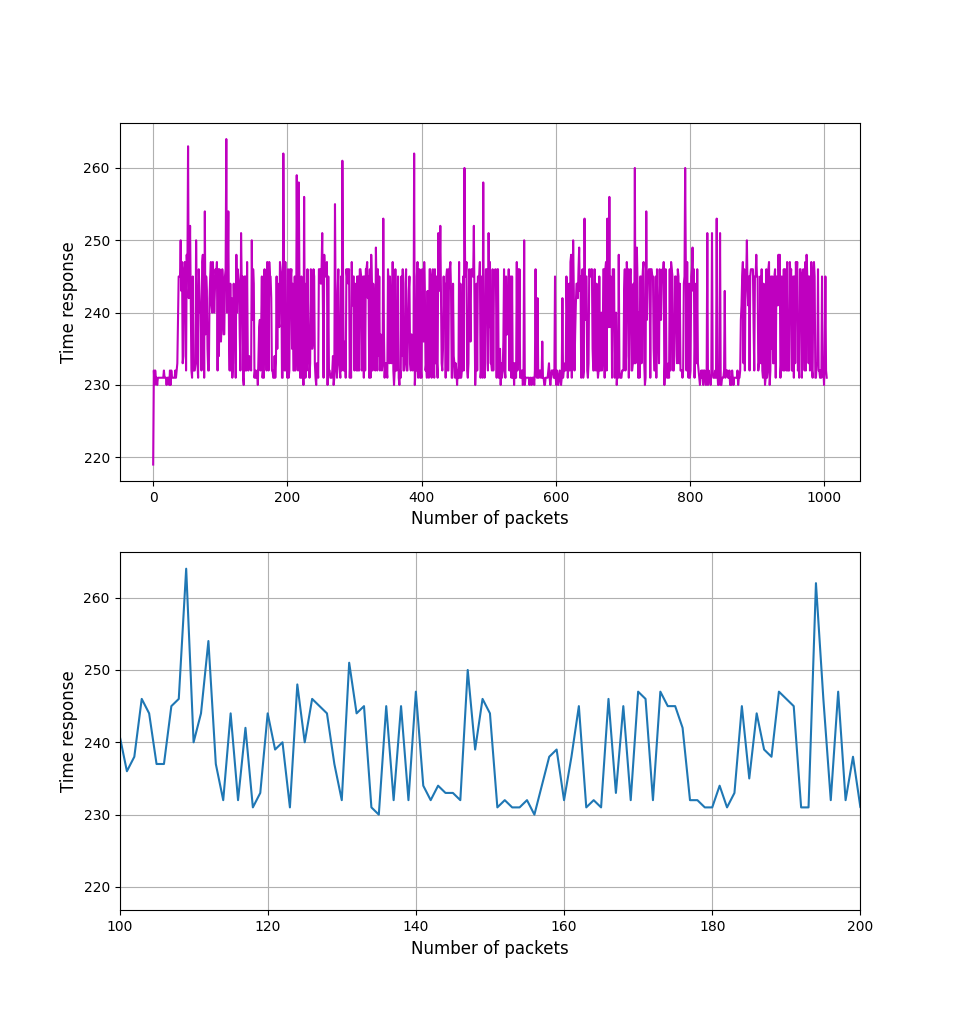
\includegraphics[height=.38\textheight, width=\textwidth]{assets/session1/g3.png}
    \caption{G3. Zoom in (below figure)} 
\end{figure}

\section{G4}

\begin{figure}[h!]
\centering
	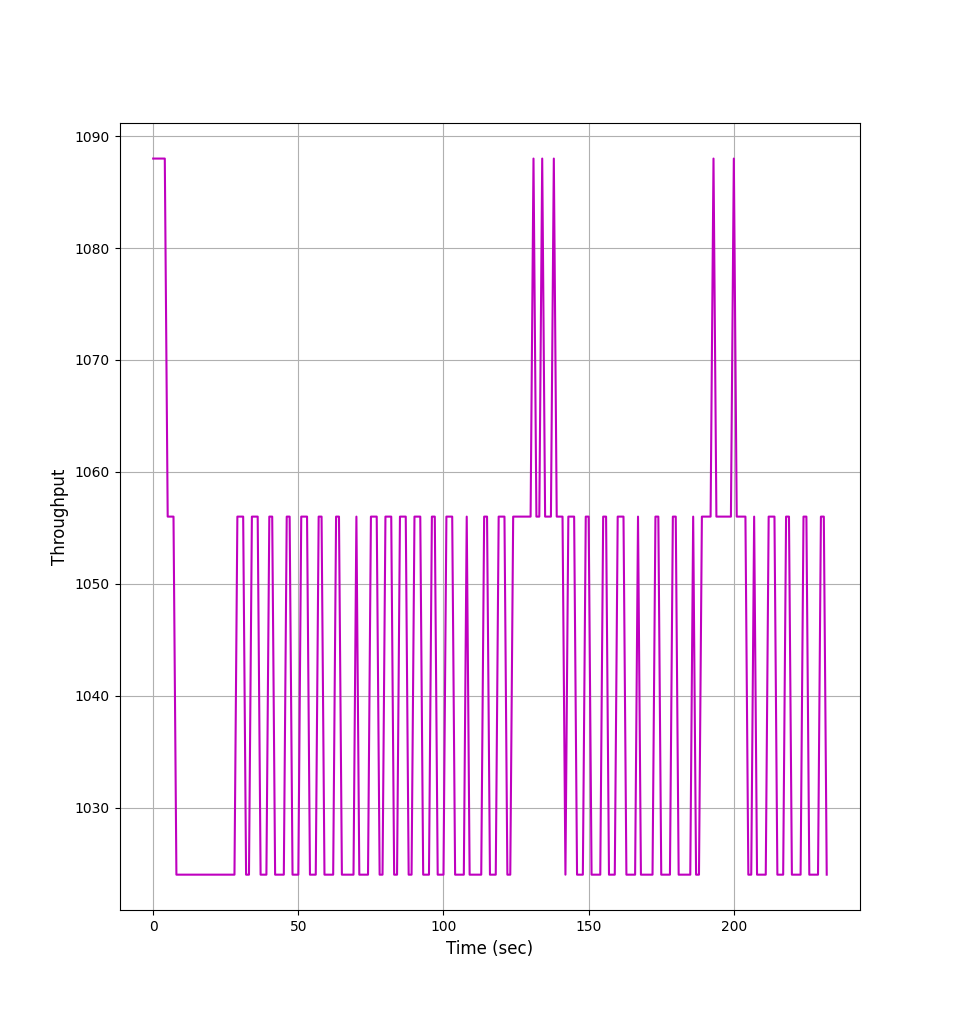
\includegraphics[height=.38\textheight, width=\textwidth]{assets/session1/g4.png}
	\caption{G4} 
\end{figure}

\section{G5}

\begin{figure}[h!]
	\centering
		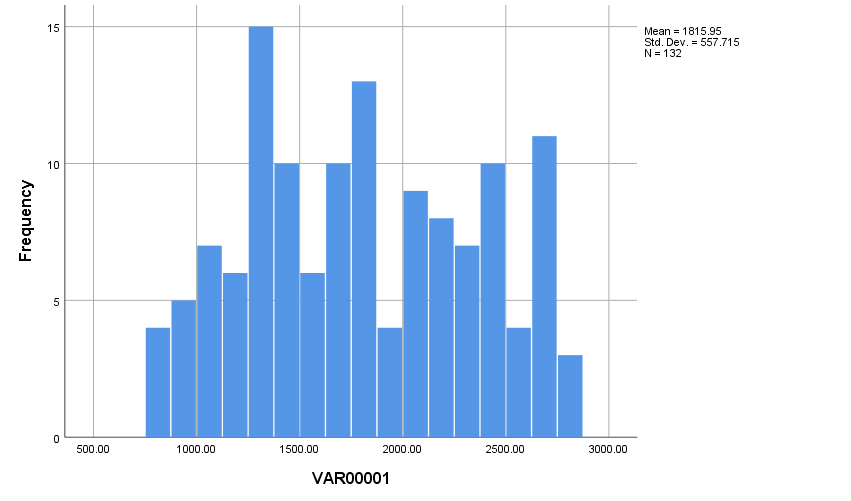
\includegraphics[height=.38\textheight, width=\textwidth]{assets/session1/g5.png}
		\caption{G5 histogram samples with delay} 
	\end{figure}

\section{G6}

\begin{figure}[h!]
	\centering
		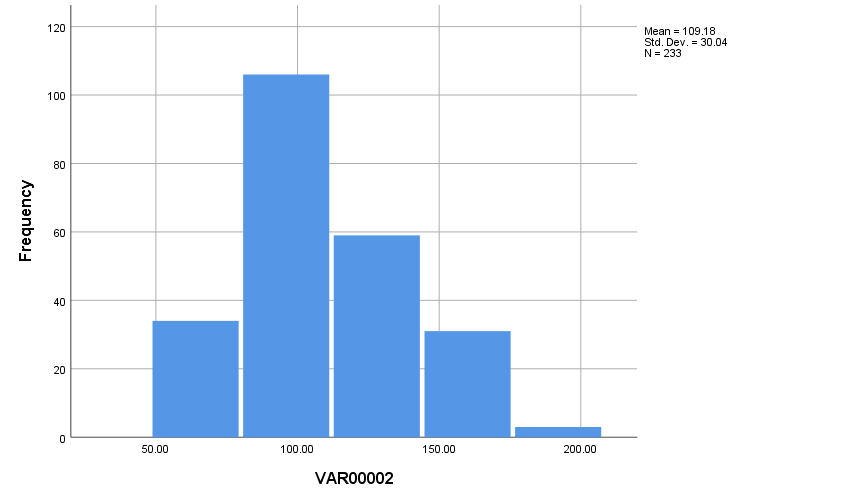
\includegraphics[height=.38\textheight, width=\textwidth]{assets/session1/g6.png}
		\caption{G5 histogram throughput with delay} 
	\end{figure}

\section{G7}

\begin{figure}[h!]
	\centering
		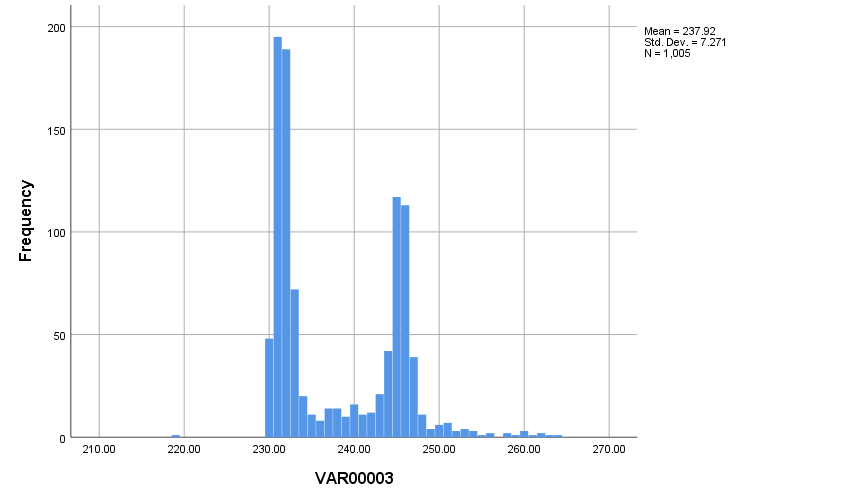
\includegraphics[height=.38\textheight, width=\textwidth]{assets/session1/g7.png}
		\caption{G5 histogram samples with no delay} 
	\end{figure}

\section{G8}

\begin{figure}[h!]
	\centering
		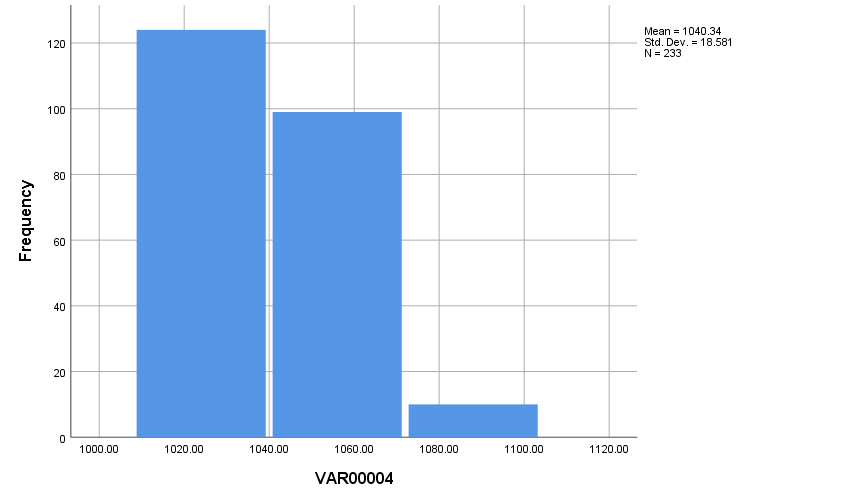
\includegraphics[height=.38\textheight, width=\textwidth]{assets/session1/g8.png}
		\caption{G5 histogram throughput with no delay} 
	\end{figure}

\section{R1}

\begin{figure}[h!]
\centering
	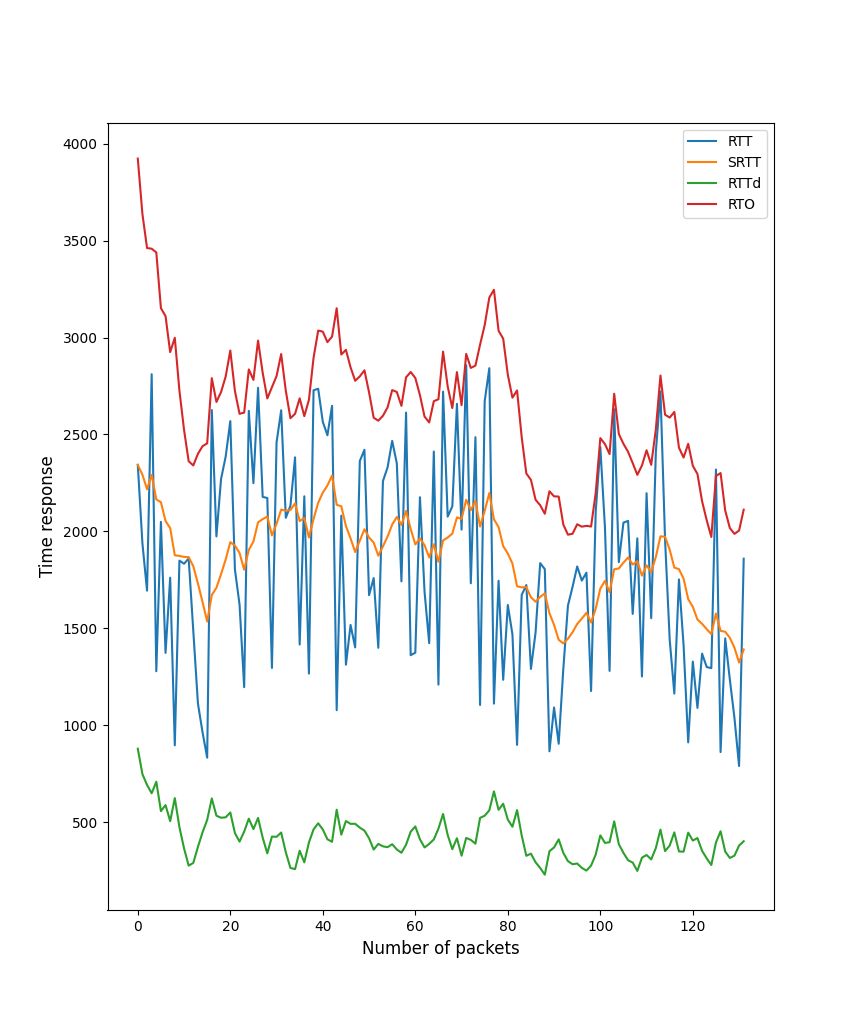
\includegraphics[height=.38\textheight, width=\textwidth]{assets/session1/r1.png}
	\caption{Retransmission timeout} 
\end{figure}

\section{Tone frequency}

\begin{figure}[h!]
\centering
	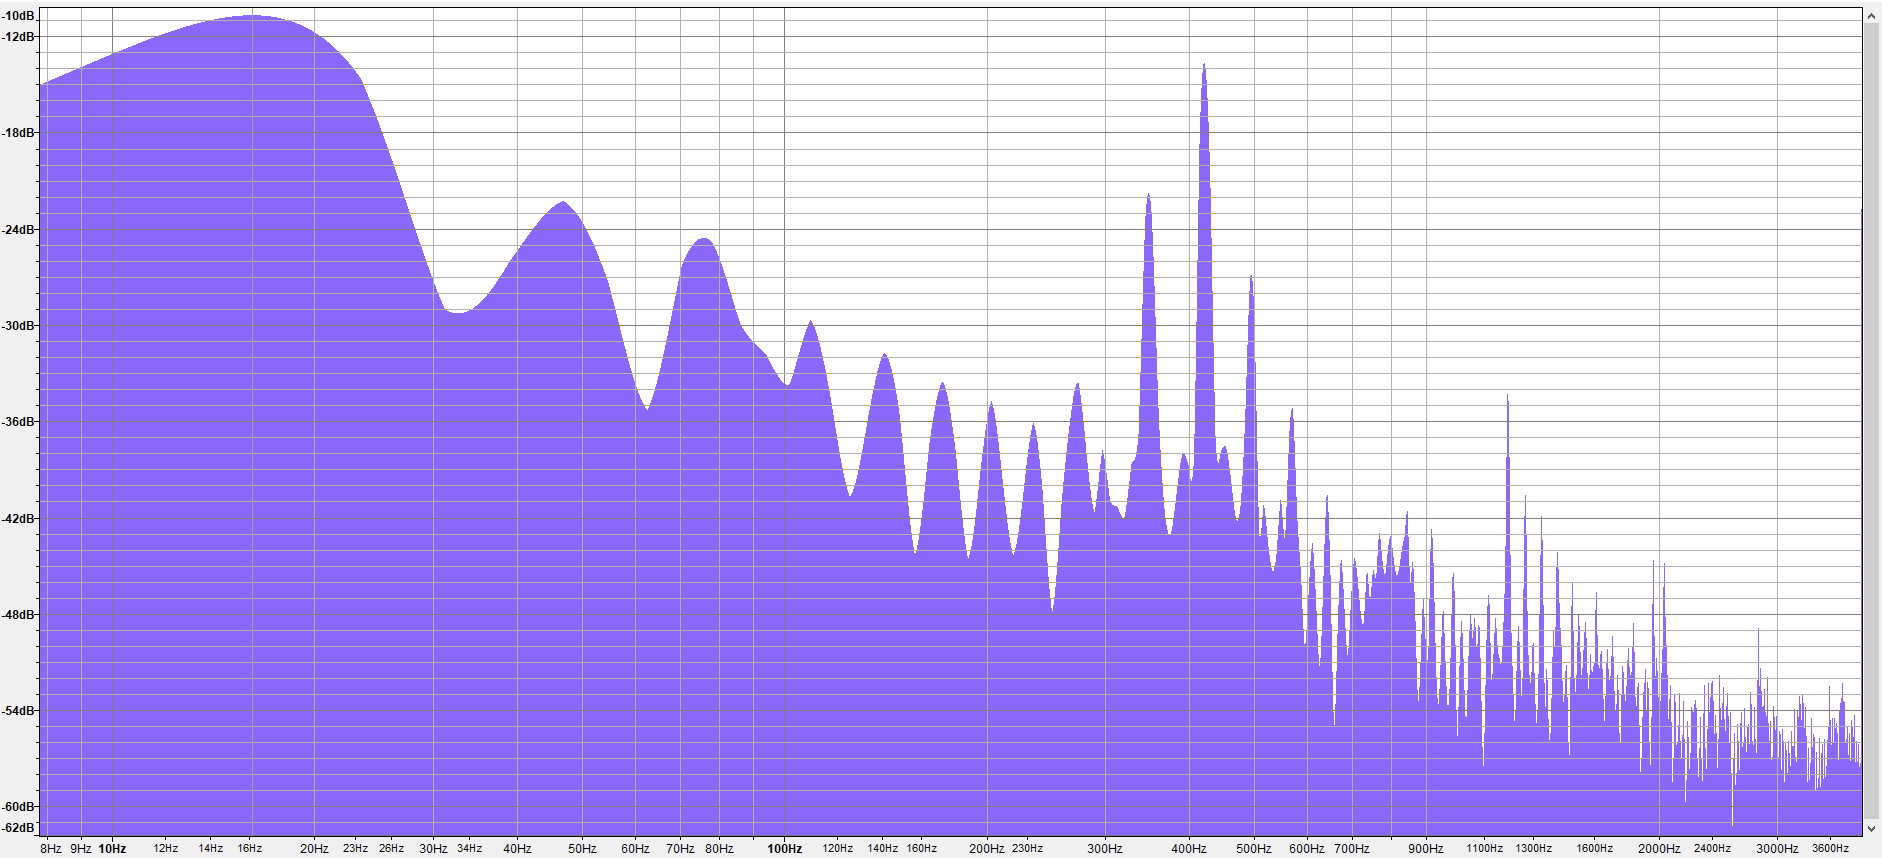
\includegraphics[height=.37\textheight, width=\textwidth]{assets/session1/spectrum.png}
    \caption{Frequency spectrum, 421 Hz and 343 Hz}
\end{figure}


\section{E1}

\begin{figure}[h!]
\centering
	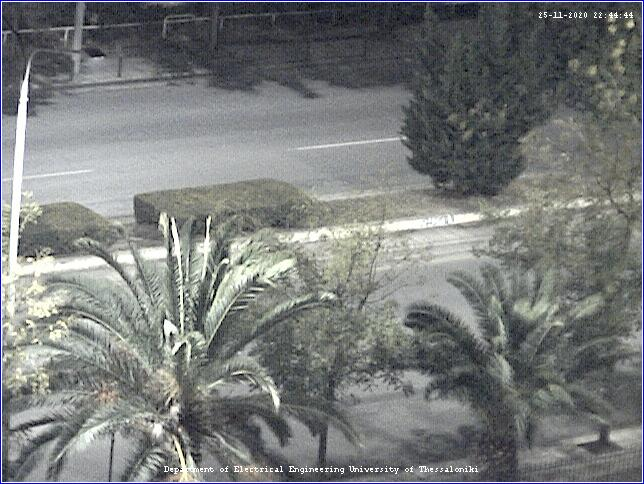
\includegraphics[height=.38\textheight, width=\textwidth]{assets/session1/image_fix.jpg}
	\caption{E1 Image code: M4898, 25/11/2020 22:44} 
\end{figure}

\section{E2}

\begin{figure}[h!]
\centering
	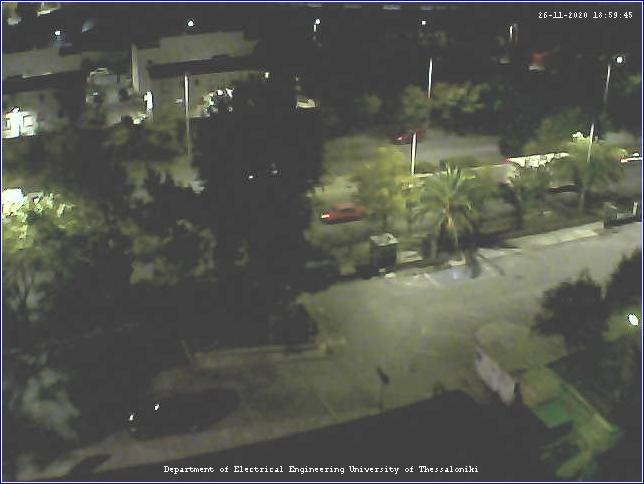
\includegraphics[height=.38\textheight, width=\textwidth]{assets/session1/image_ptz.jpg}
	\caption{E2 Image code:M5983CAM=PTZ} 
\end{figure}
CAM=PTZ
M5983 
2020-11-26T18:54:05.822247
2020-11-26T18:54:07.481316

Το στρίψαμε και λίγο γιατι έδειχνε στον τοίχο. Αξίζει να σημειωθεί οτι χρειάζεται να επέλθει καποιος χρόνος για να γίνει το readjust.
Παρατηρούμε ότι σε αυτήν την κάμερα υπάρχει ένα offset 4-5 λεπτών απο αυτήν που απεικονίζεται στην εικόνα. Δοκιμάζοντας το για αρκετές εικόνες φαίνεται όντως να ιυπάρχει μια καθυστέρηση σε εκείνο το ρολόι σε σχέση με το FIX

\section{Temperature}

\begin{figure}[h!]
\centering
	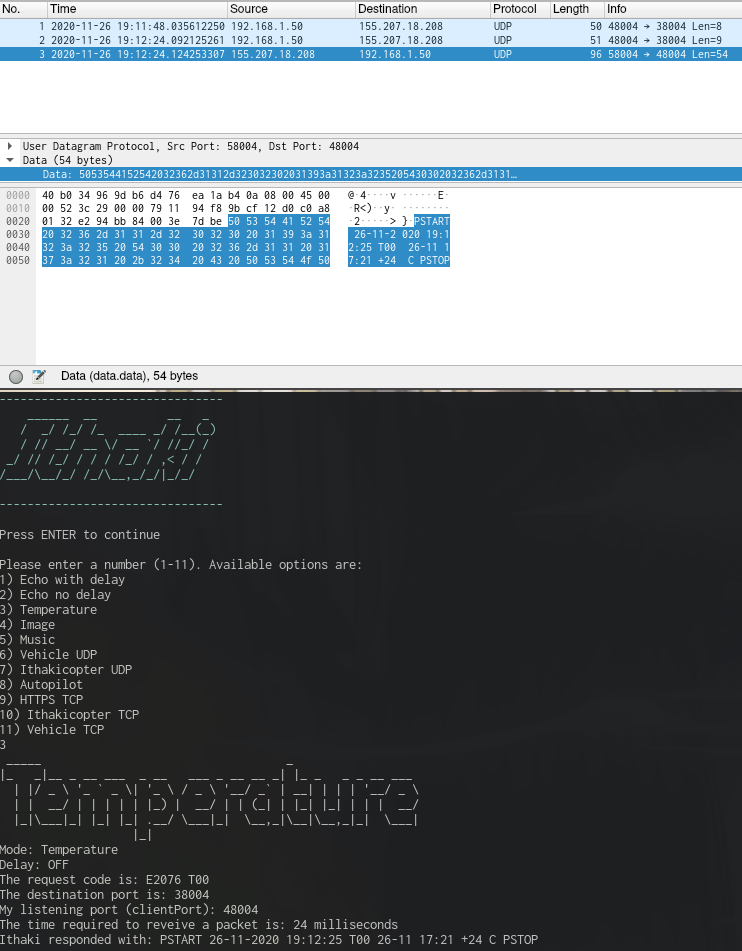
\includegraphics[height=.38\textheight, width=.8\textwidth]{assets/session1/temp.png}
	\caption{Temperature} 
\end{figure}
Request code: E2076 T00
Info Temperature app:
2020-11-26T19:12:24.081612
2020-11-26T19:12:24.132789


\section{G9}

\begin{figure}[h!]
\centering
	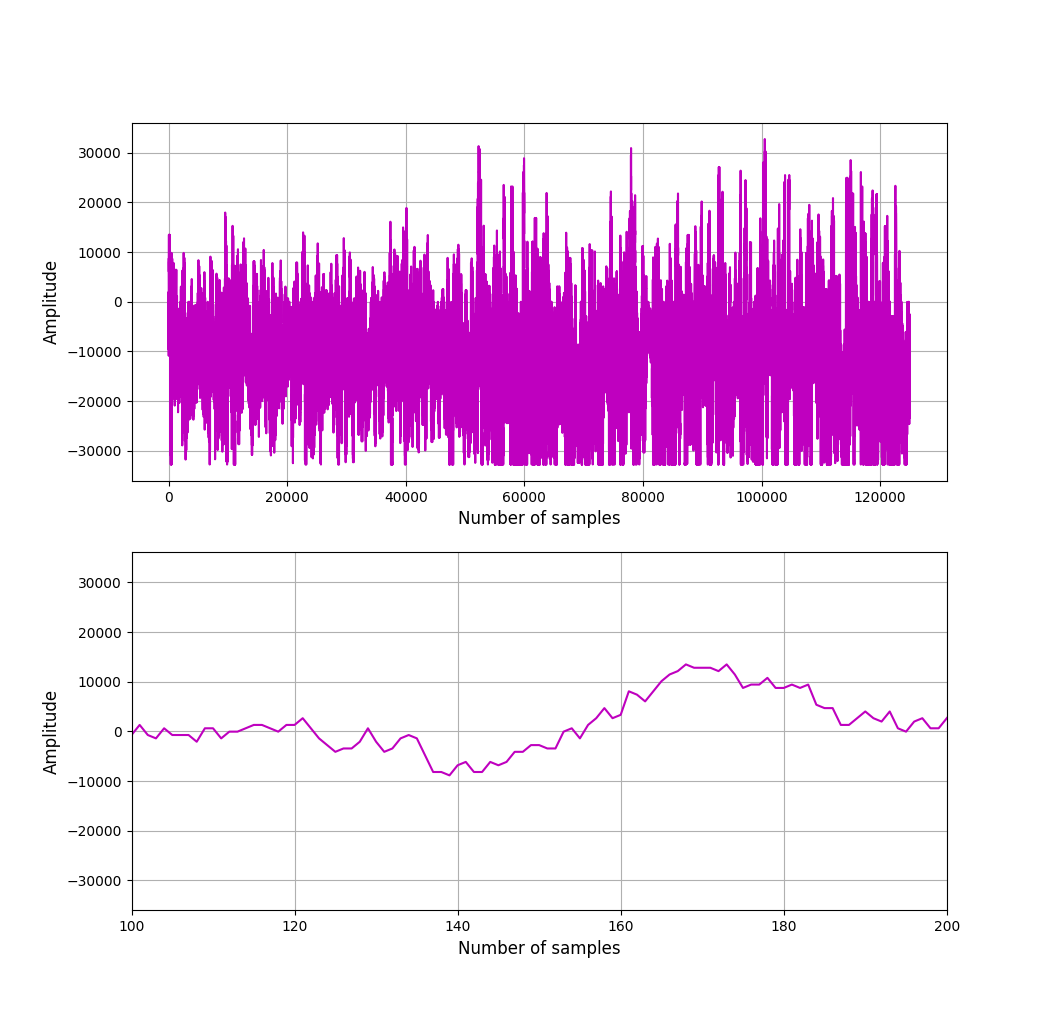
\includegraphics[height=.38\textheight, width=\textwidth]{assets/session1/g9_aq.png}
	\caption{G9 AQDPCM samples waveform, code: L22A8610AQF500, time: 25/11/2020 22:47} 
\end{figure}


\section{G10}

\begin{figure}[h!]
\centering
	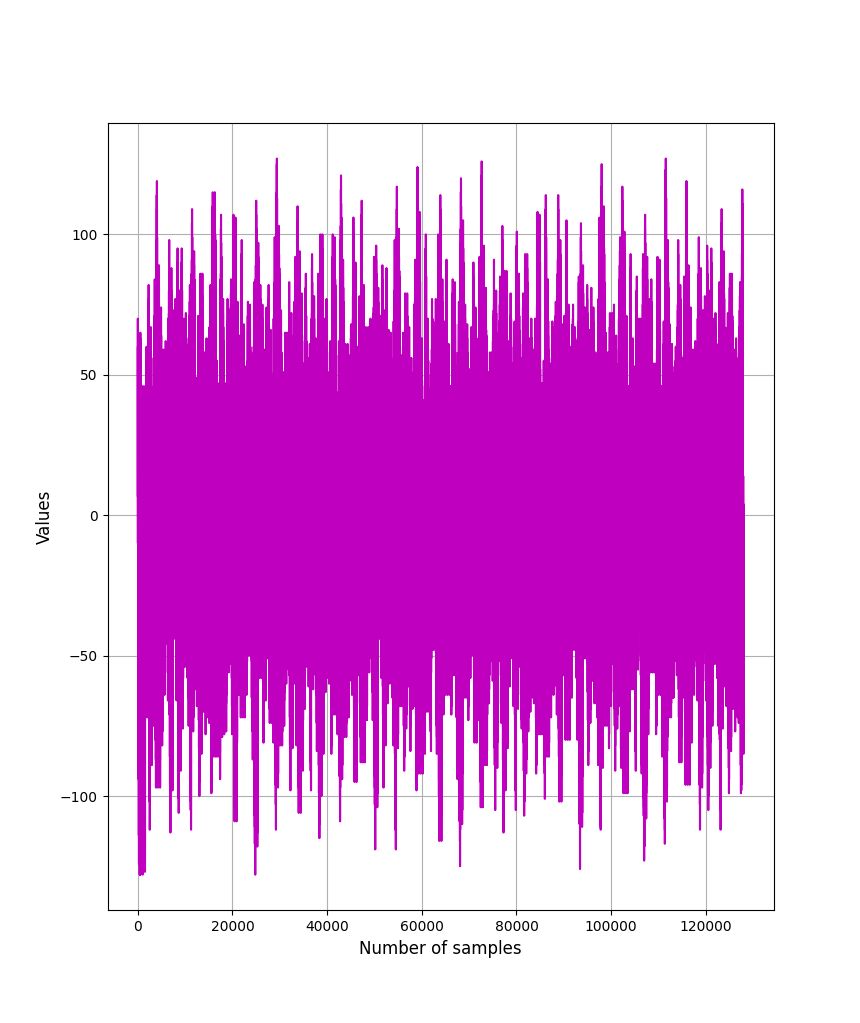
\includegraphics[height=.38\textheight, width=\textwidth]{assets/session1/g10.png}
    \caption{G10 DPCM samples waveform Tone,2020-11-26T02:14:33.921607, code: A1275 DPCM Type:T}
\end{figure}

\section{G11}
2020-11-26T02:45:47.961502
2020-11-26T02:46:23.588615
code: A1275 AQDPCM type F, L22
\begin{figure}[h!]
\centering
	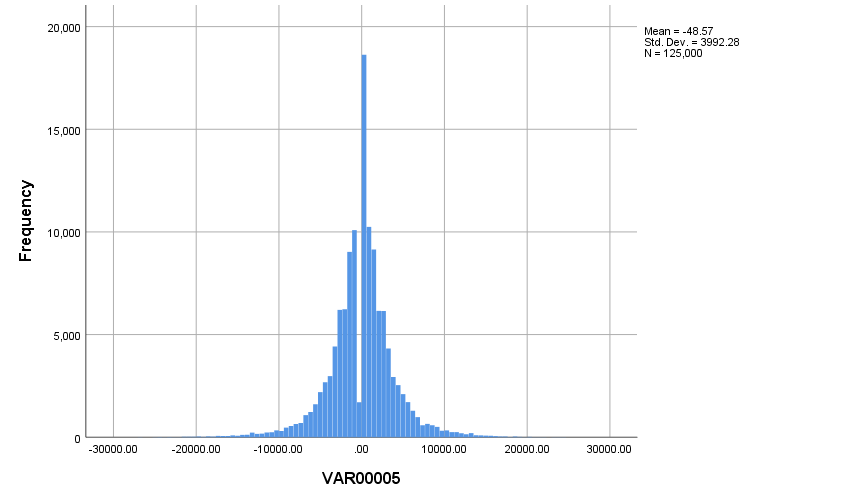
\includegraphics[height=.38\textheight, width=\textwidth]{assets/session1/g11.png}
    \caption{G11 AQDPCM diff samples}
\end{figure}

\section{G12}

\begin{figure}[h!]
	\centering
		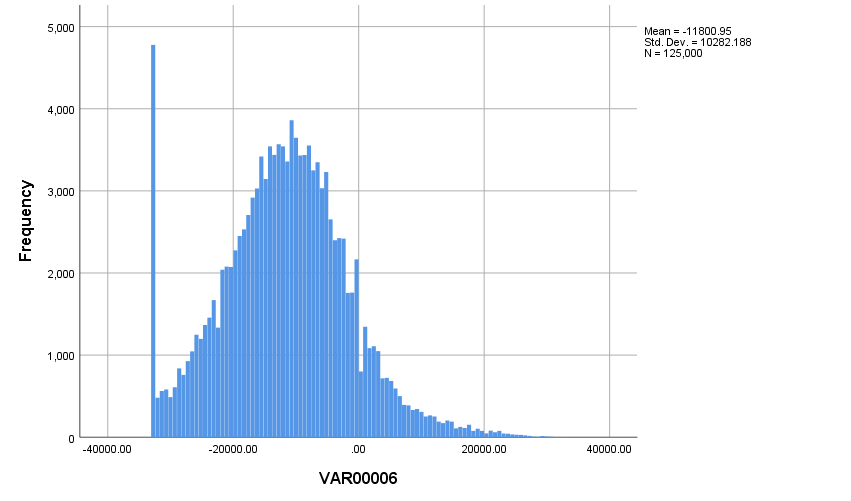
\includegraphics[height=.38\textheight, width=\textwidth]{assets/session1/g12.png}
		\caption{G12 AQDPCM  samples}
	\end{figure}

\section{G13}
DPCM type F
2020-11-26T02:41:10.482168
2020-11-26T02:41:46.461623
code: A1275 L22 
\begin{figure}[h!]
	\centering
		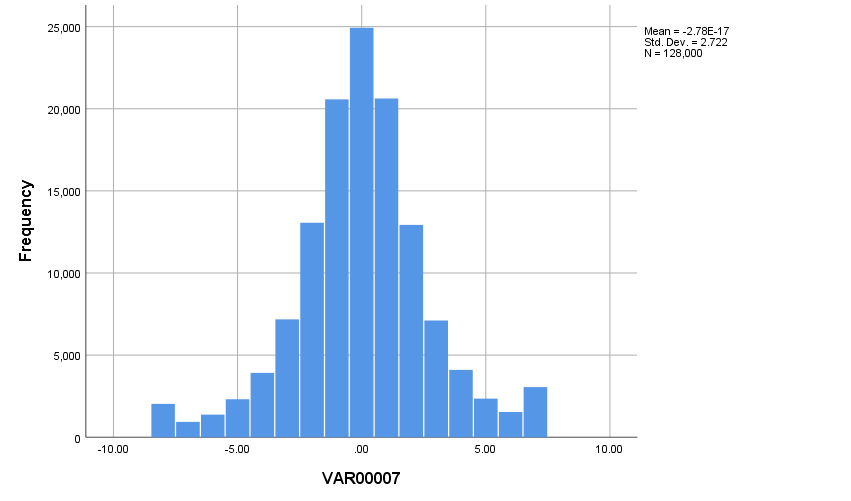
\includegraphics[height=.38\textheight, width=\textwidth]{assets/session1/g13.png}
		\caption{G13 DPCM diff samples}
	\end{figure}

\section{G14}
\begin{figure}[h!]
	\centering
		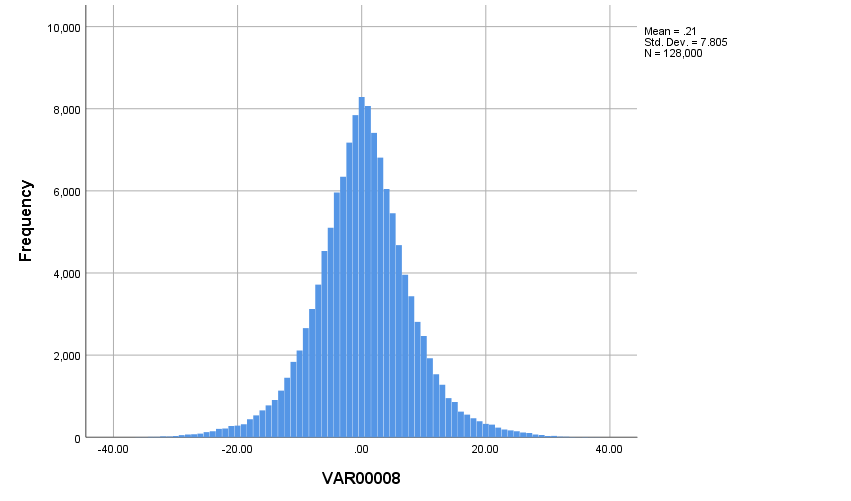
\includegraphics[height=.38\textheight, width=\textwidth]{assets/session1/g14.png}
		\caption{G14 DPCM  samples}
	\end{figure}

\section{G15}

\begin{figure}[h!]
\centering
	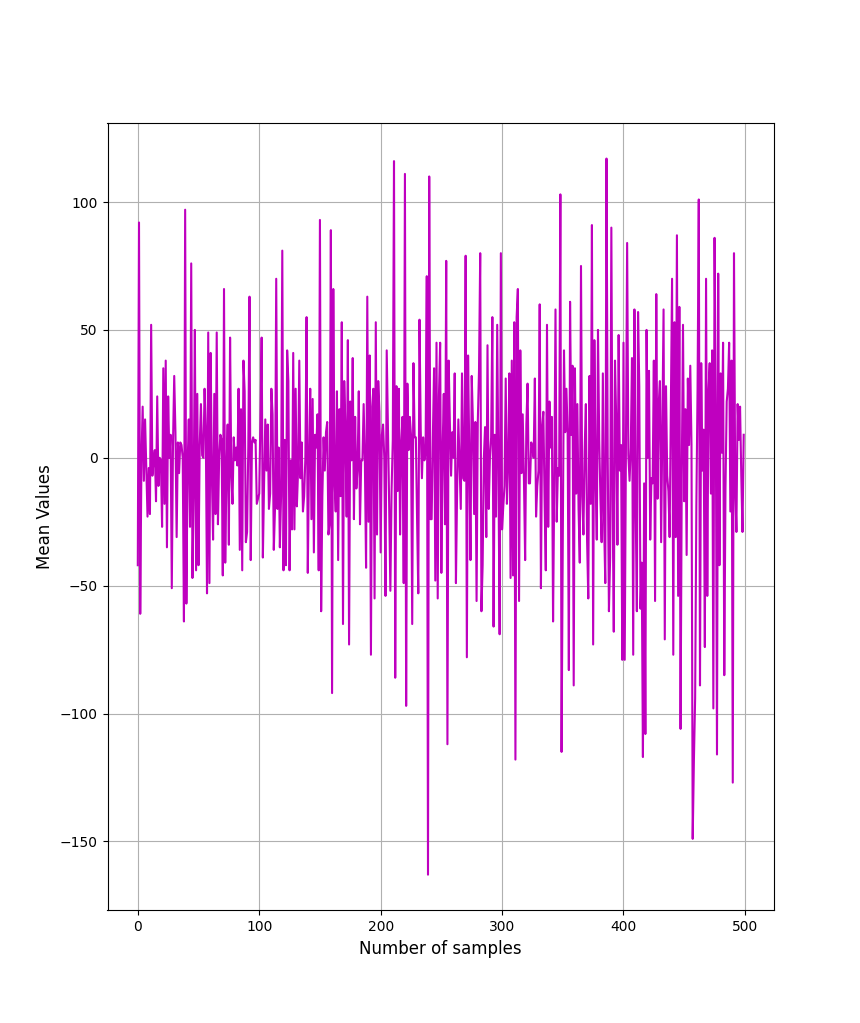
\includegraphics[height=.38\textheight, width=\textwidth]{assets/session1/g15.png}
    \caption{G15 Mean 1st clip 2020-11-26T02:45:47.961502, code: A1275 AQDPCM Type:F, L22}
\end{figure}

\section{G16}

\begin{figure}[h!]
\centering
	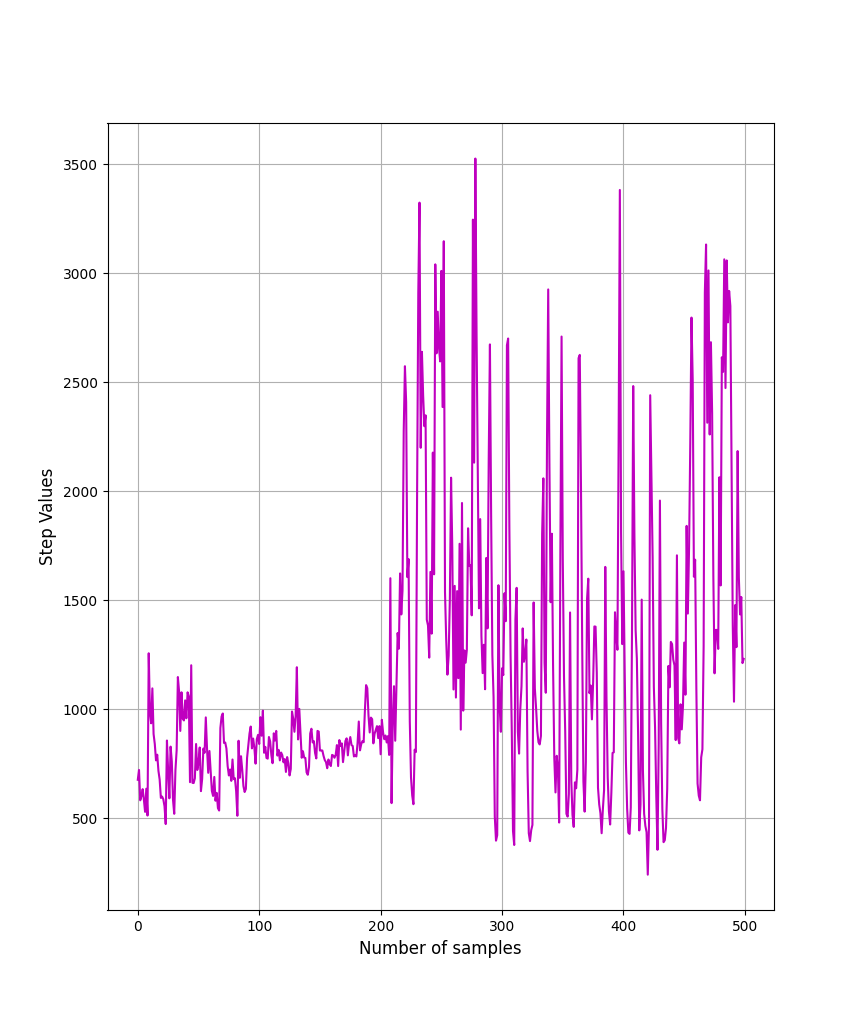
\includegraphics[height=.38\textheight, width=\textwidth]{assets/session1/g16.png}
    \caption{G16 Step 1st clip  2020-11-26T02:45:47.961502 code: A1275 AQDPCM Type:F, L22}
\end{figure}

\section{G17}
%L11 AQDPCM type F
%time: 2020-11-26T14:45:39.638111
%2020-11-26T14:46:15.252079

\begin{figure}[h!]
\centering
	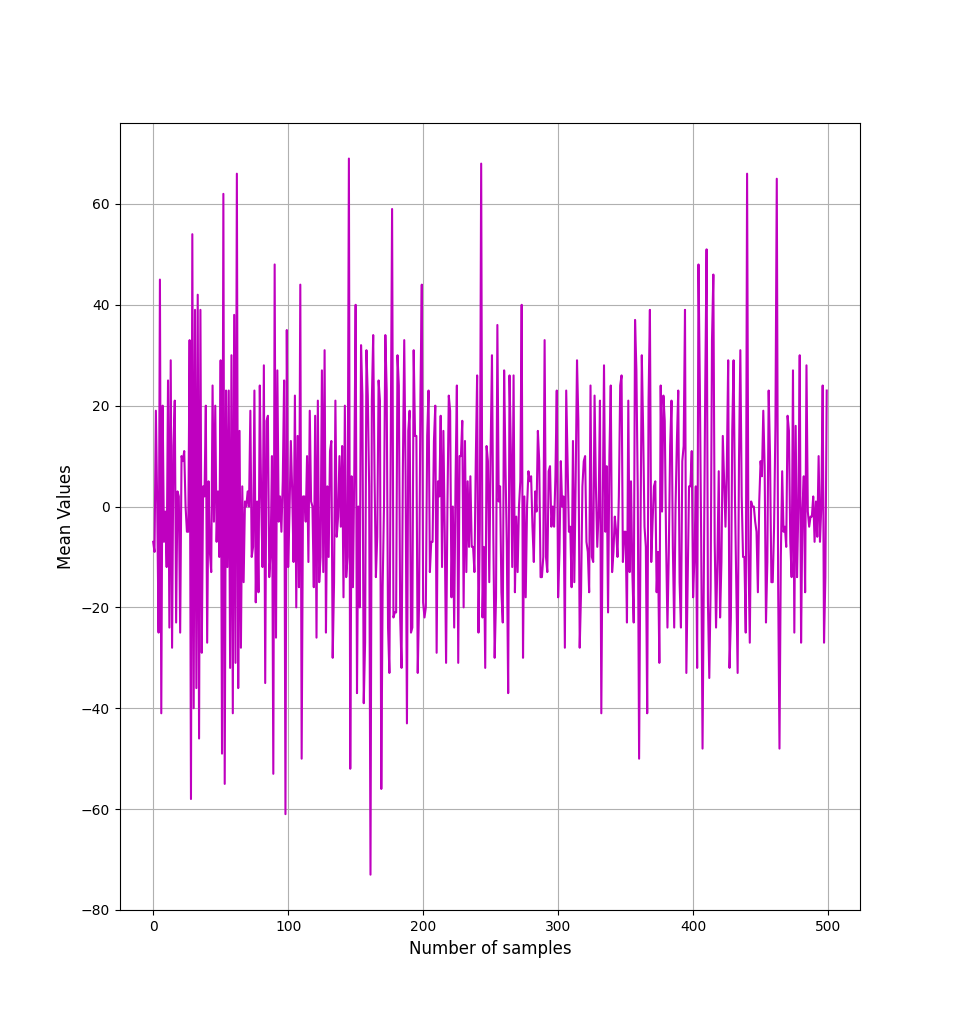
\includegraphics[height=.38\textheight, width=\textwidth]{assets/session1/g17.png}
    \caption{G17 Mean 2nd clip  2020-11-26T14:45:39.638111 L11 AQDPCM type F}
\end{figure}



\section{G18}

\begin{figure}[h!]
\centering
	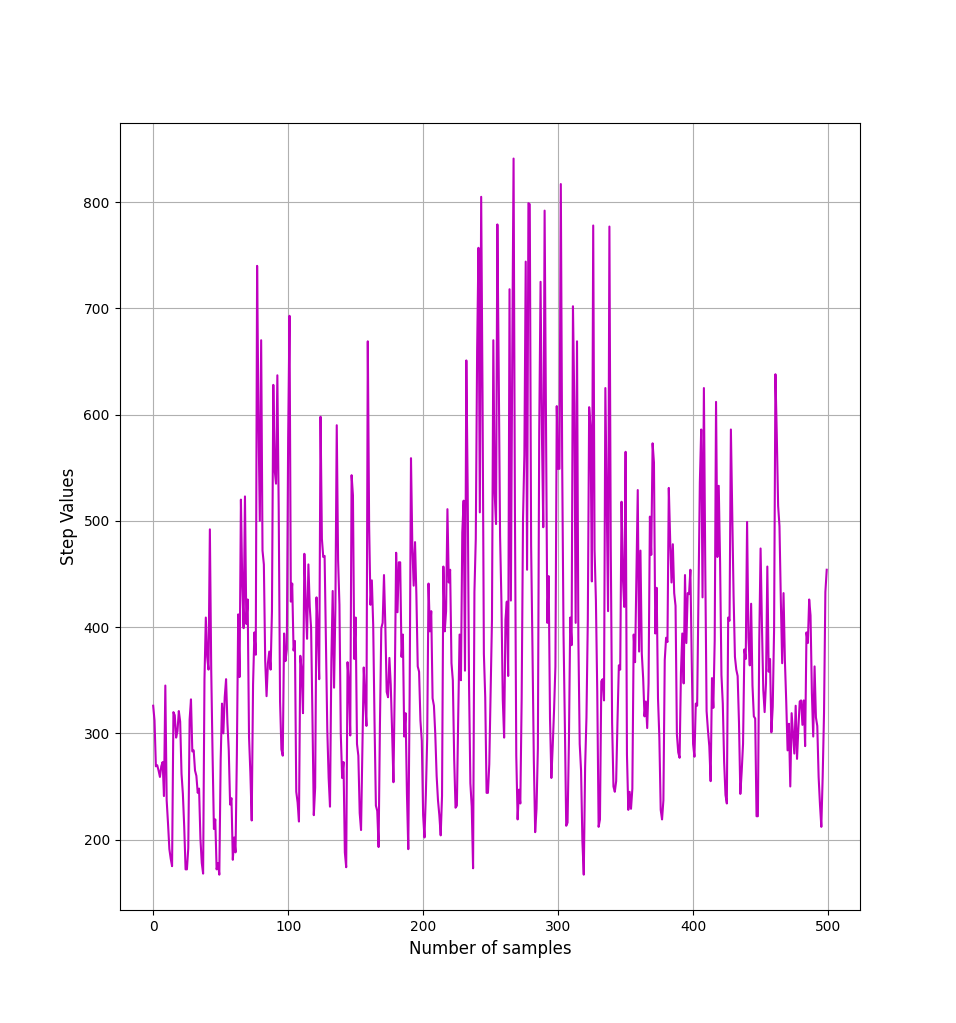
\includegraphics[height=.38\textheight, width=\textwidth]{assets/session1/g18.png}
    \caption{G18 Step 2nd clip   2020-11-26T14:45:39.638111  L11 AQDPCM type F}
\end{figure}



\section{G19}
Πρώτη μέτρηση
Info Ithakicopter app:
2020-11-25T22:56:19.083780
2020-11-25T22:57:09.811613

\begin{figure}[h!]
\centering
	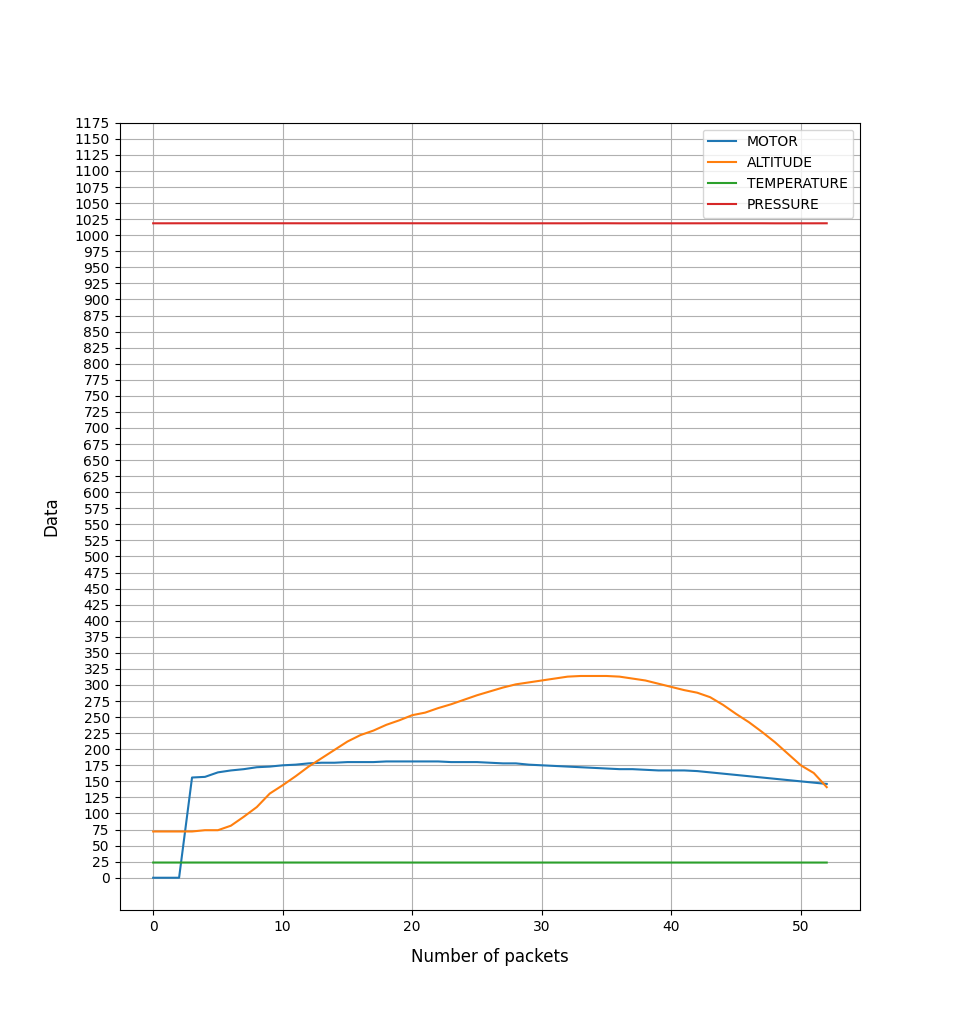
\includegraphics[height=.4\textheight, width=\textwidth]{assets/session1/g19.png}
    \caption{G19 Flightlevel περίπου 300}
\end{figure}

\section{G20}

\begin{figure}[h!]
\centering
	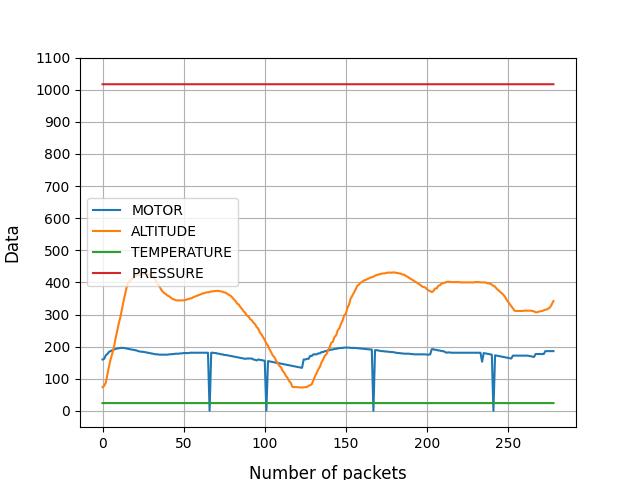
\includegraphics[height=.4\textheight, width=\textwidth]{assets/session1/g20.png}
    \caption{G20 Flightlevel περίπου 400}
\end{figure}
Info Ithakicopter app:
2020-11-26T19:26:39.407225
2020-11-26T19:27:57.238542

Μια αρκετά πιο ενδιαφέρουσα προσέγγιση αφήνοντας να τρέξει το copter λιγο παραπάνω παρατηρούμε την προσπάθεα του autopilot παρά τις πιθανόν διάφορες εντολές που λαμβάνει απο άλλους χρήστες να προσπαθεί να πιάσει το επιθυμητό flightlevel

\section{G21}

Info Vehicle app:
2020-11-25T22:58:42.235997
2020-11-25T23:02:42.512168

\begin{figure}[h!]
\centering
	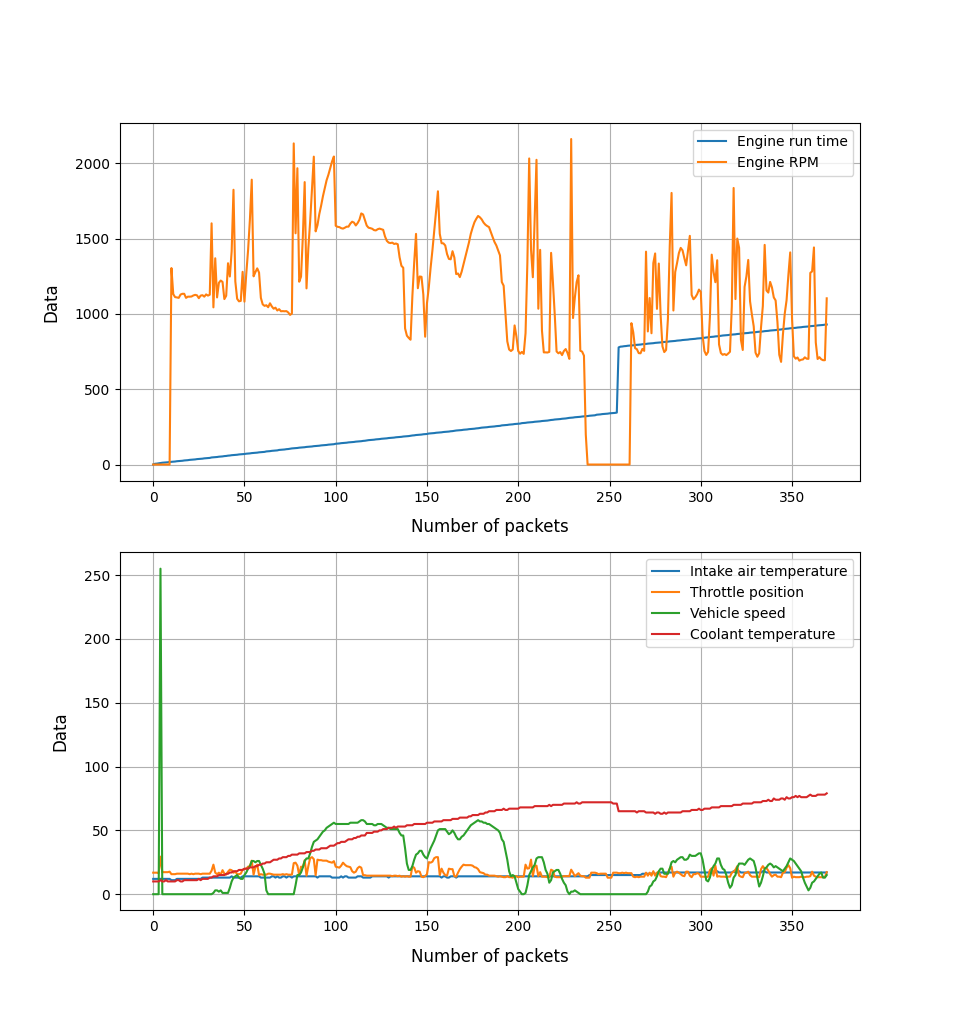
\includegraphics[height=.5\textheight, width=\textwidth]{assets/session1/g21.png}
    \caption{G21 Vehicle OBD}
\end{figure}

\end{document}
